%%%%%%%%%%%%%%%%%%%%%%%%%%%%%%%%%%%%%%%%%%%%%%%%%%%%%%%%%%%%%%%%%%%%%%
\section{Introduction}

%%%%%%%%%%%%%%%%%%%%%%%%%%%%%%%%%%%%%%%%%%
\subsection{The distributional hypothesis}

\begin{frame}[c]
  \frametitle{Meaning \& distribution}
  % \framesubtitle{}

  \begin{itemize}
  \item ``Die Bedeutung eines Wortes liegt in seinem Gebrauch.''\\
    \hfill --- Ludwig Wittgenstein
  \item[]\pause
  \item ``You shall know a word by the company it keeps!''\\
    \hfill --- J.~R.\ \citet{Firth:57}
  \item[]\pause
  \item Distributional hypothesis \citep[Zellig][]{Harris:54}
  \end{itemize}
\end{frame}

\begin{frame}
  \frametitle{What is the meaning of ``\textbf{bardiwac}''?}
  % \framesubtitle{}

  \begin{itemize}
  \item<2-> He handed her her glass of \primary{bardiwac}.
  \item<3-> Beef dishes are made to complement the \primary{bardiwacs}.
  \item<4-> Nigel staggered to his feet, face flushed from too much \primary{bardiwac}.
  \item<5-> Malbec, one of the lesser-known \primary{bardiwac} grapes, responds well to Australia's sunshine.
  \item<6-> I dined off bread and cheese and this excellent \primary{bardiwac}.
  \item<7-> The drinks were delicious: blood-red \primary{bardiwac} as well as light, sweet Rhenish.
  \item[\hand]<8-> bardiwac is a heavy red alcoholic beverage made from grapes
  \end{itemize}
\end{frame}

\begin{frame}[c]
  \frametitle{Real-life concordance \& word sketch}
  \framesubtitle{http://beta.sketchengine.co.uk/}

  \begin{center}
    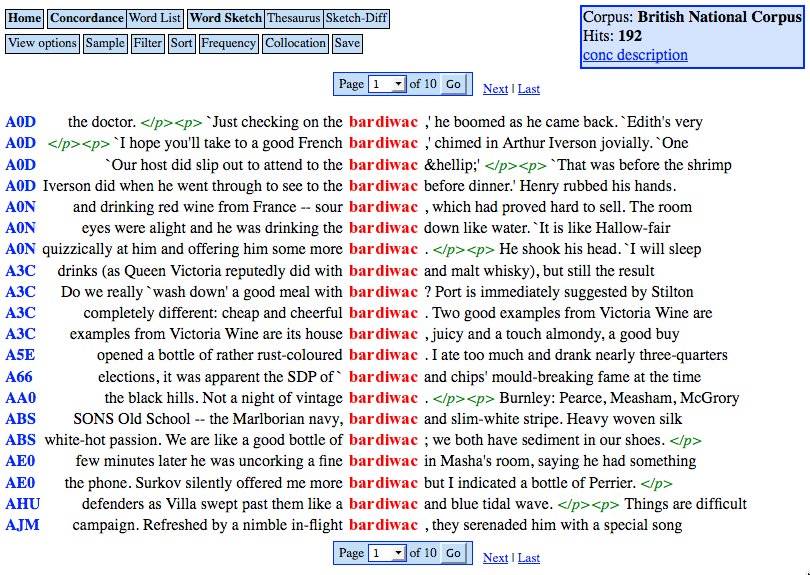
\includegraphics[width=10cm]{img/SE_bardiwac_conc}
  \end{center}
\end{frame}

\begin{frame}[c]
  \frametitle{Real-life concordance \& word sketch}
  \framesubtitle{http://beta.sketchengine.co.uk/}

  \begin{center}
    \ungap[1]
    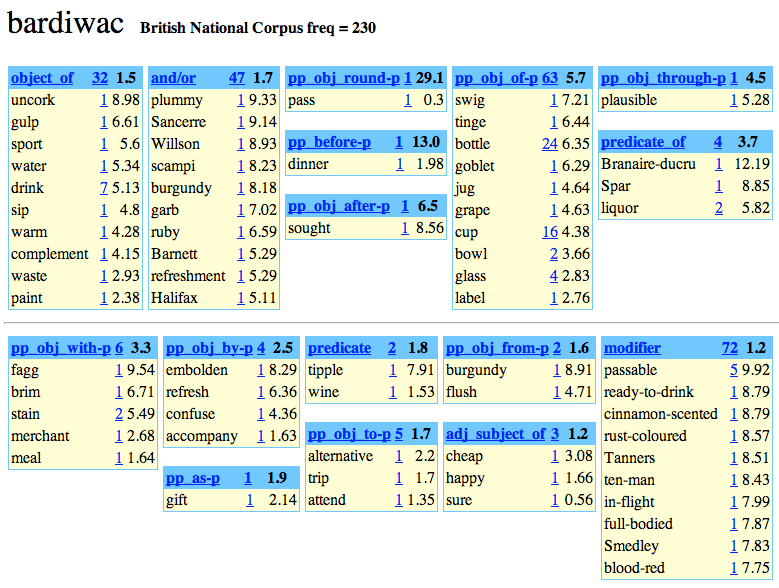
\includegraphics[width=10cm]{img/SE_bardiwac_sketch}
  \end{center}
\end{frame}

{\newcommand{\hg}[1]{\scriptsize\textpmhg{#1}}
\begin{frame}<beamer:1-4| handout:1-4>
  \frametitle{A thought experiment: deciphering hieroglyphs}
  % \framesubtitle{}

  \begin{center}
    \setlength{\arrayrulewidth}{1pt}
    \begin{tabular}{@{\rule{0mm}{1.2em} }lr*{6}{|c}|}
      && \hg{get} & \hg{sij} & \hg{ius} & \hg{hir} & \hg{iit} & \hg{kil} \\
      \hline
      \secondary<beamer:2| handout:2>{(knife)} & \secondary<beamer:2| handout:2>{\hg{naif}} & \secondary<beamer:2| handout:2>{51} & \secondary<beamer:2| handout:2>{20} & \secondary<beamer:2| handout:2>{84} &  \secondary<beamer:2| handout:2>{0} &  \secondary<beamer:2| handout:2>{3} &  \secondary<beamer:2| handout:2>{0} \\
      \hline
      \secondary<beamer:4| handout:4>{(cat)}   & \secondary<beamer:4| handout:4>{\hg{ket}}  &  \secondary<beamer:4| handout:4>{52} & \secondary<beamer:4| handout:4>{58} &  \secondary<beamer:4| handout:4>{4} &  \secondary<beamer:4| handout:4>{4} &  \secondary<beamer:4| handout:4>{6} & \secondary<beamer:4| handout:4>{26} \\
      \hline
      \h{???} & \h{\hg{dog}} & \primary{115} & \primary{83} & \primary{10} & \primary{42} & \primary{33} & \primary{17} \\
      \hline
      (boat)  & \hg{beut} &  59 & 39 & 23 &  4 &  0 &  0 \\
      \hline
      (cup)   & \hg{kap}  &  98 & 14 &  6 &  2 &  1 &  0 \\
      \hline
      \secondary<beamer:3| handout:3>{(pig)}  & \secondary<beamer:3| handout:3>{\hg{pigij}} &  \secondary<beamer:3| handout:3>{12} & \secondary<beamer:3| handout:3>{17} &  \secondary<beamer:3| handout:3>{3} &  \secondary<beamer:3| handout:3>{2} &  \secondary<beamer:3| handout:3>{9} & \secondary<beamer:3| handout:3>{27} \\
      \hline
      (banana) & \hg{nana} & 11 &  2 &  2 &  0 & 18 &  0 \\
      \hline
    \end{tabular}
    
    \gap[2]\Large
    \only<beamer:2| handout:2>{%
      sim(\primary{\hg{dog}}, \secondary{\hg{naif}}) = 0.770 }%
    \only<beamer:3| handout:3>{%
      sim(\primary{\hg{dog}}, \secondary{\hg{pigij}}) = 0.939 }%
    \only<beamer:4| handout:4>{%
      sim(\primary{\hg{dog}}, \secondary{\hg{ket}}) = 0.961 }%
  \end{center}

  \addnote{Similarity scores are cosine similarities on sparse log-scaled frequencies ($\log (f+1)$).}%
\end{frame}
}

{\newcommand{\hg}[1]{\scriptsize\textpmhg{#1}}
\begin{frame}
  \frametitle{English as seen by the computer \ldots}
  % \framesubtitle{}

  \begin{center}
    \ungap[1]
    \setlength{\arrayrulewidth}{1pt}
    \begin{tabular}{@{\rule{0mm}{1.2em} }l@{ }r*{6}{|c}|}
      && get & see & use & hear & eat & kill \\
      && \hg{get} & \hg{sij} & \hg{ius} & \hg{hir} & \hg{iit} & \hg{kil} \\
      \hline
      knife & \hg{naif} &  51 & 20 & 84 &  0 &  3 &  0 \\
      \hline
      cat   & \hg{ket}  &  52 & 58 &  4 &  4 &  6 & 26 \\
      \hline
      \h{dog} & \h{\hg{dog}} & \primary{115} & \primary{83} & \primary{10} & \primary{42} & \primary{33} & \primary{17} \\
      \hline
      boat  & \hg{beut} &  59 & 39 & 23 &  4 &  0 &  0 \\
      \hline
      cup   & \hg{kap}  &  98 & 14 &  6 &  2 &  1 &  0 \\
      \hline
      pig  & \hg{pigij} &  12 & 17 &  3 &  2 &  9 & 27 \\
      \hline
      banana & \hg{nana} & 11 &  2 &  2 &  0 & 18 &  0 \\
      \hline
    \end{tabular}
  \end{center}
  \hfill\light{\footnotesize verb-object counts from British National Corpus}
\end{frame}
}

\begin{frame}
  \frametitle{Geometric interpretation}
  % \framesubtitle{}

  \begin{columns}[T]
    \begin{column}{40mm}
      \begin{itemize}
      \item row vector \primary{$\vx_{\text{dog}}$} describes usage of word \emph{dog} in the corpus
      \item can be seen as coordinates of point in $n$-dimensional Euclidean space
       \end{itemize}
    \end{column}
    \begin{column}{75mm}      
      \gap[2]
      \begin{small}
        \setlength{\arrayrulewidth}{1pt}
        \begin{tabular}{r*{6}{|c}|}
          & get & see & use & hear & eat & kill \\
          \hline
          knife &  51 & 20 & 84 &  0 &  3 &  0 \\
          \hline
          cat  &  52 & 58 &  4 &  4 &  6 & 26 \\
          \hline
          \h{dog} & \primary{115} & \primary{83} & \primary{10} & \primary{42} & \primary{33} & \primary{17} \\
          \hline
          boat &  59 & 39 & 23 &  4 &  0 &  0 \\
          \hline
          cup  &  98 & 14 &  6 &  2 &  1 &  0 \\
          \hline
          pig  &  12 & 17 &  3 &  2 &  9 & 27 \\
          \hline
          banana & 11 &  2 &  2 &  0 & 18 &  0 \\
          \hline
        \end{tabular}
      \end{small}

      \begin{center}
        \h{co-occurrence matrix} $M$
      \end{center}
    \end{column}
  \end{columns}
\end{frame}

\begin{frame}
  \frametitle{Geometric interpretation}
  % \framesubtitle{}

  \begin{columns}[T]
    \begin{column}{40mm}
      \begin{itemize}
      \item row vector \primary{$\vx_{\text{dog}}$} describes usage of word \emph{dog} in the corpus
      \item can be seen as coordinates of point in $n$-dimensional Euclidean space
      \item illustrated for two dimensions:\\ \emph{get} and \emph{use}
      \item \primary{$\vx_{\text{dog}} = (115,10)$}
      \end{itemize}
    \end{column}
    \begin{column}{75mm}      
      \ungap[1]
      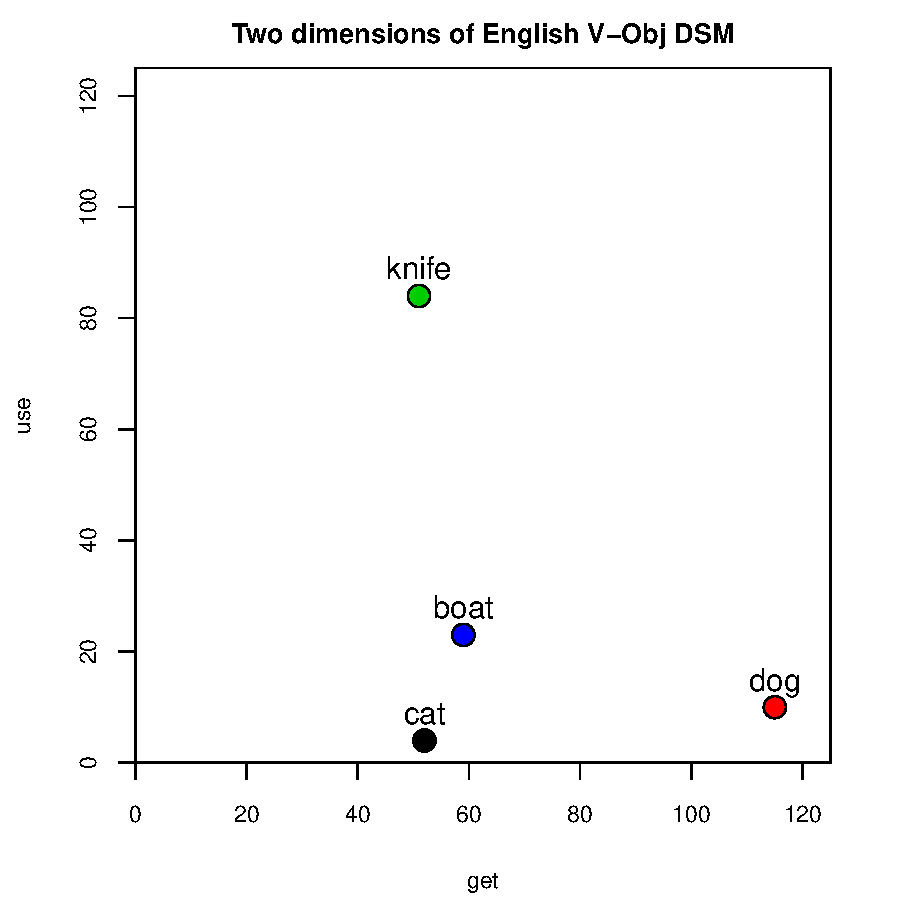
\includegraphics[width=75mm]{img/hieroglyph_2d_1}
    \end{column}
  \end{columns}
\end{frame}

\begin{frame}
  \frametitle{Geometric interpretation}
  % \framesubtitle{}

  \begin{columns}[T]
    \begin{column}{40mm}
      \begin{itemize}
      \item similarity = spatial proximity (Euclidean dist.)
      \item location depends on frequency of noun ($f_{\text{dog}} \approx 2.7\cdot f_{\text{cat}}$)
      \end{itemize}
    \end{column}
    \begin{column}{75mm}      
      \ungap[1]
      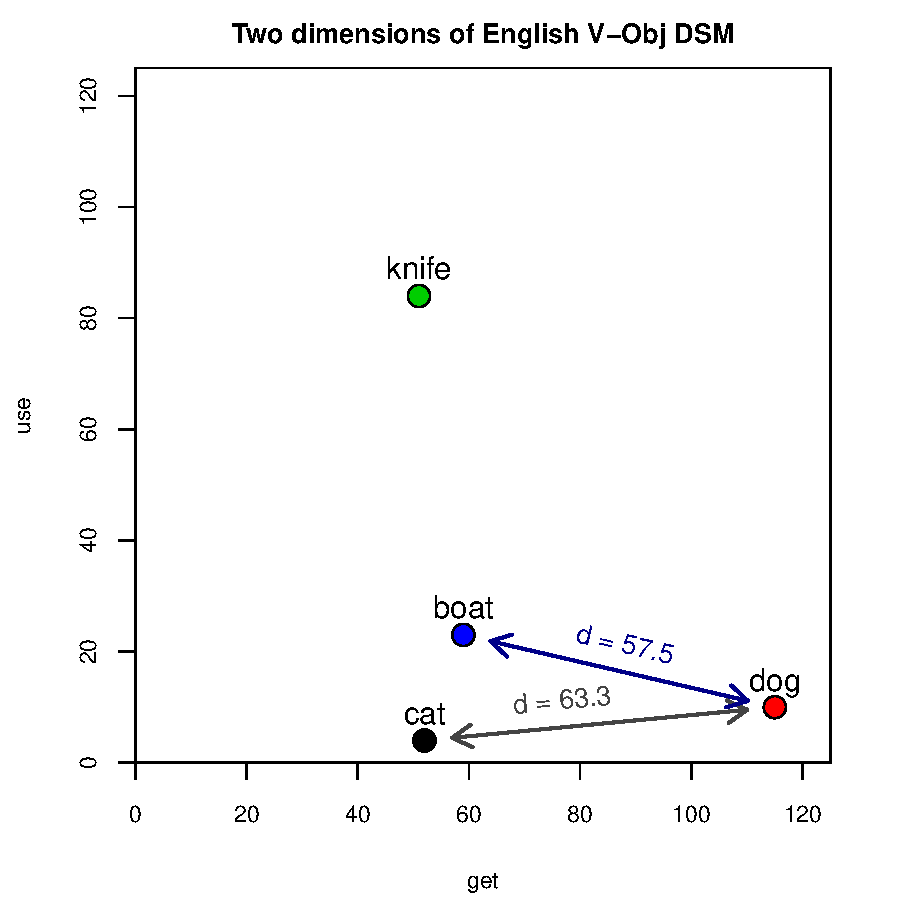
\includegraphics[width=75mm]{img/hieroglyph_2d_2}
    \end{column}
  \end{columns}
\end{frame}

\begin{frame}
  \frametitle{Geometric interpretation}
  % \framesubtitle{}

  \begin{columns}[T]
    \begin{column}{40mm}
      \begin{itemize}
      \item similarity = spatial proximity (Euclidean dist.)
      \item location depends on frequency of noun ($f_{\text{dog}} \approx 2.7\cdot f_{\text{cat}}$)
      \item direction more important than location
      \end{itemize}
    \end{column}
    \begin{column}{75mm}      
      \ungap[1]
      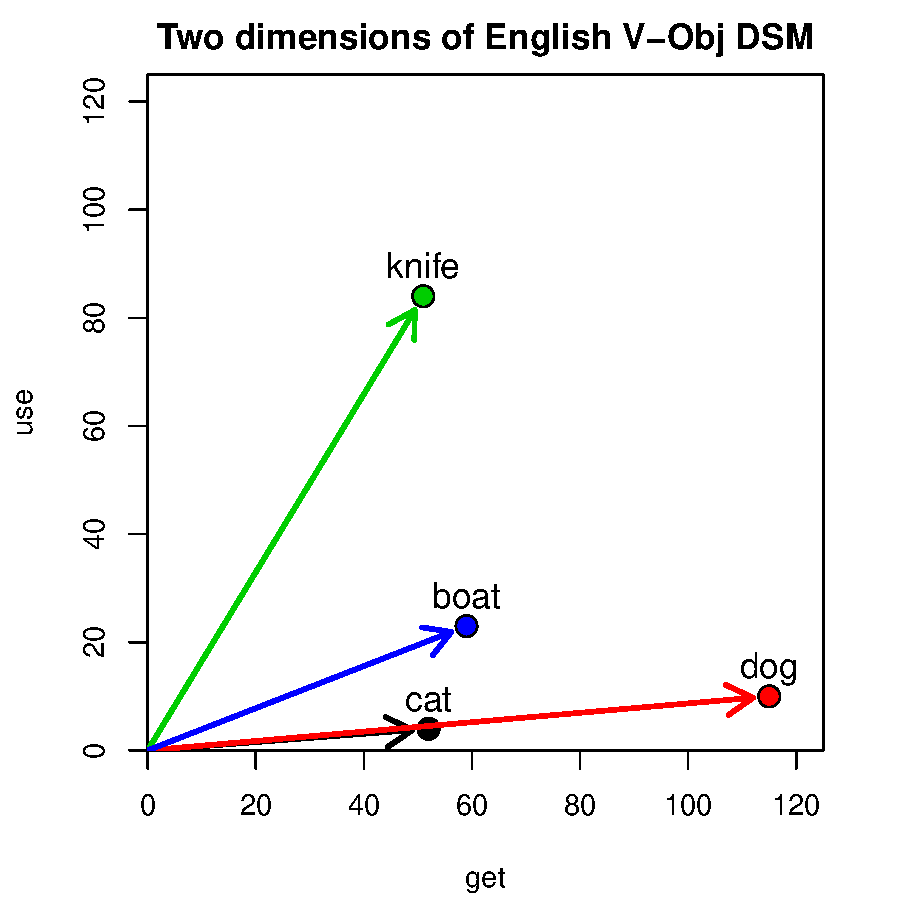
\includegraphics[width=75mm]{img/hieroglyph_2d_3}
    \end{column}
  \end{columns}
\end{frame}

\begin{frame}
  \frametitle{Geometric interpretation}
  % \framesubtitle{}

  \begin{columns}[T]
    \begin{column}{40mm}
      \begin{itemize}
      \item similarity = spatial proximity (Euclidean dist.)
      \item location depends on frequency of noun ($f_{\text{dog}} \approx 2.7\cdot f_{\text{cat}}$)
      \item direction more important than location
      \item<1-> normalise ``length'' $\norm{\vx_{\text{dog}}}$ of vector
      \item<2-> or use angle $\alpha$ as distance measure
      \end{itemize}
    \end{column}
    \begin{column}{75mm}
      \ungap[1]
      \only<beamer:1| handout:0>{%
        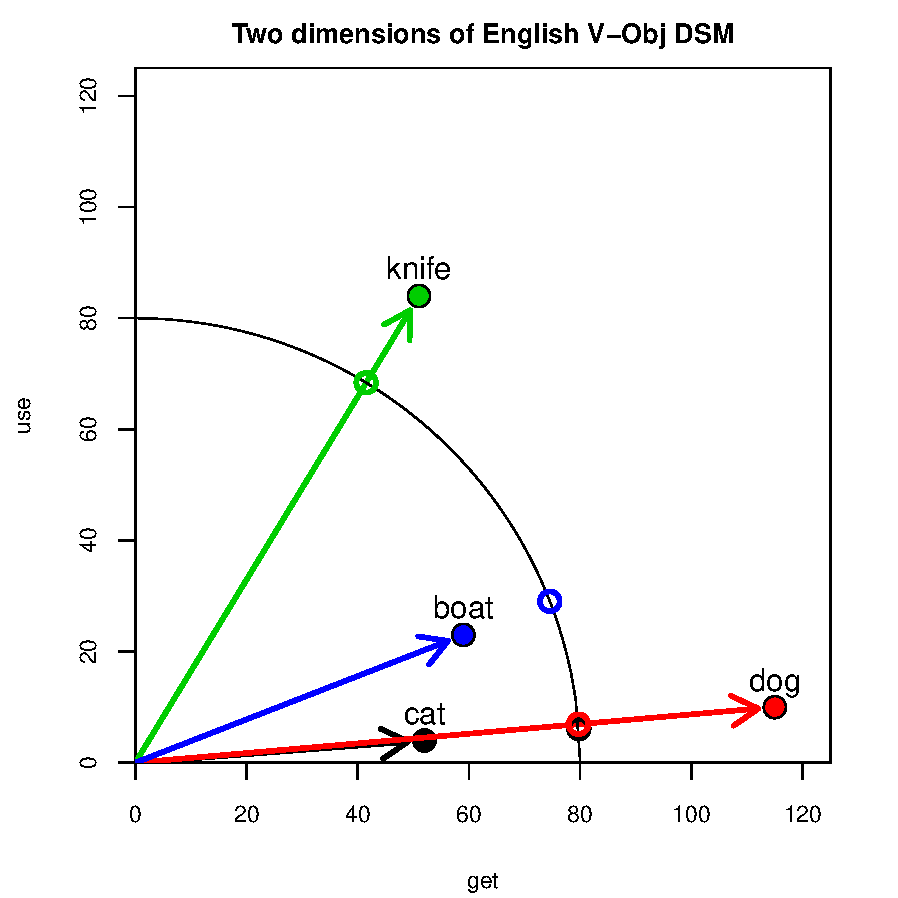
\includegraphics[width=75mm]{img/hieroglyph_2d_4}}%
      \only<beamer:2| handout:1>{%
        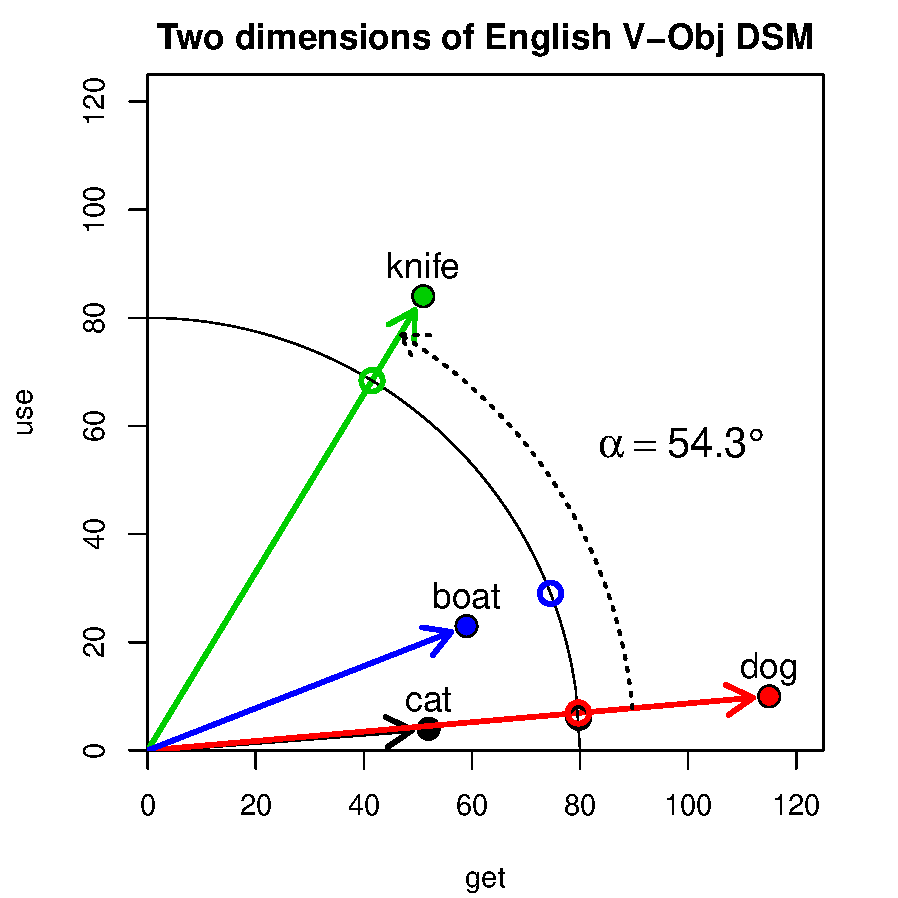
\includegraphics[width=75mm]{img/hieroglyph_2d_5}}%
    \end{column}
  \end{columns}
\end{frame}

\begin{frame}
  \frametitle{Semantic distances}
  % \framesubtitle{}

  \begin{columns}[T]
    \begin{column}{55mm}
      \begin{itemize}
      \item main result of distributional analysis are ``semantic'' distances between words
      \item typical applications
        \begin{itemize}
        \item nearest neighbours
        \item clustering of related words
        \item construct semantic map
        \end{itemize}
      \end{itemize}
    \end{column}
    \begin{column}{55mm}
      \ungap[1]
      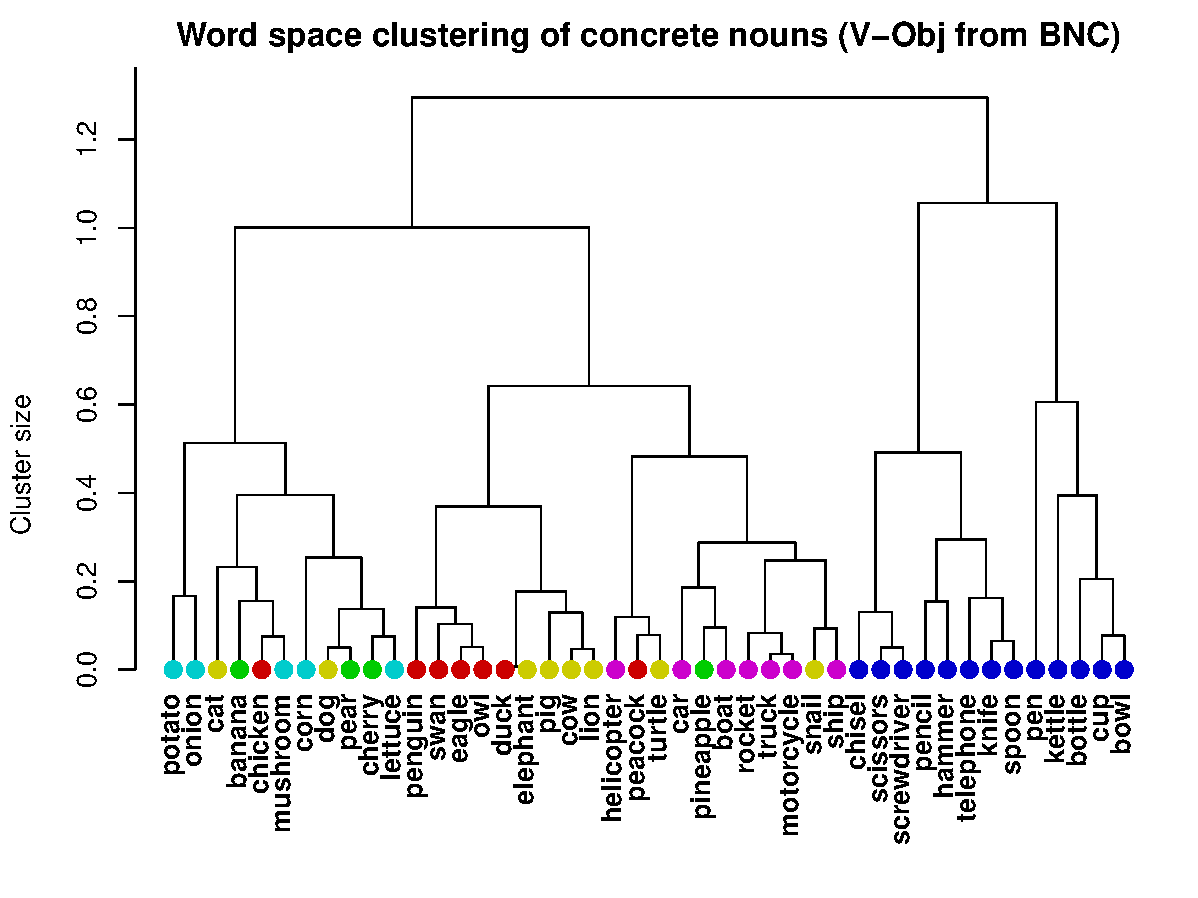
\includegraphics[width=50mm]{img/hieroglyph_clustering}

      \gap[1]
      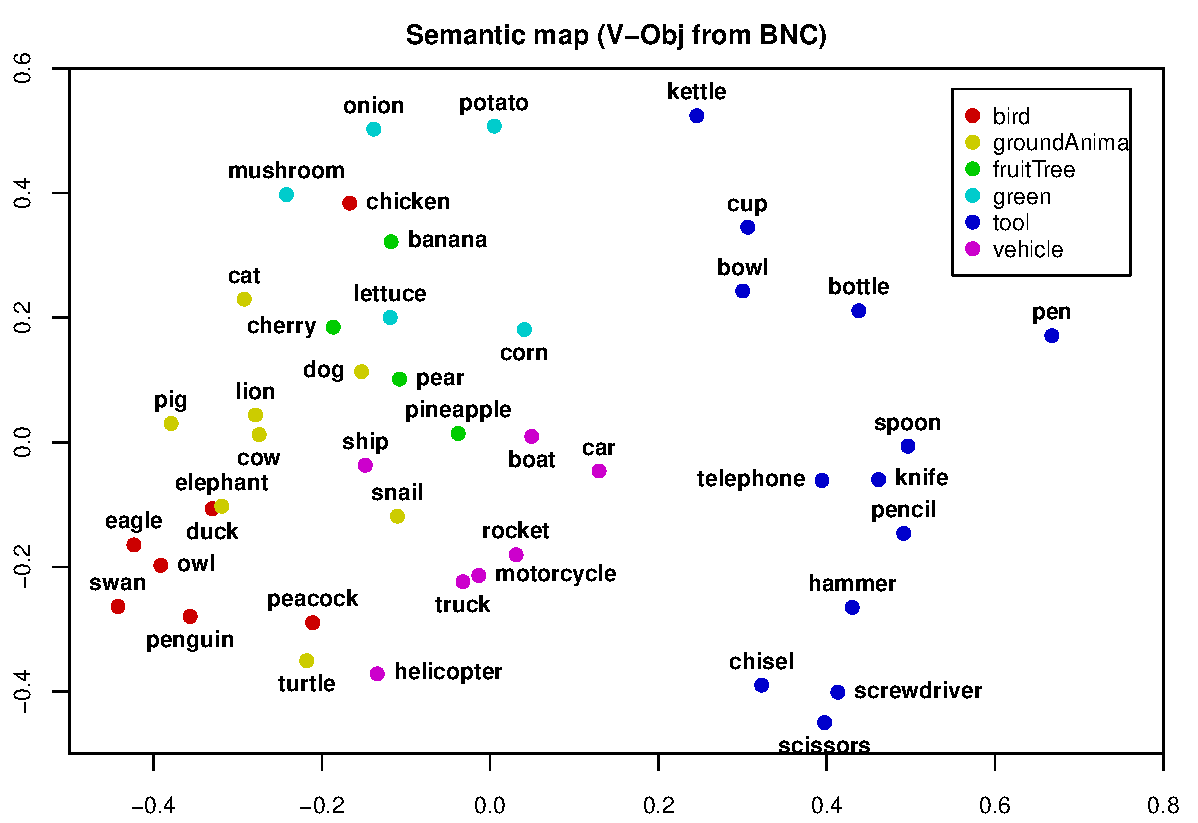
\includegraphics[width=50mm]{img/hieroglyph_semantic_map}
    \end{column}
  \end{columns}
\end{frame}

%%%%%%%%%%%%%%%%%%%%%%%%%%%%%%%%%%%%%%%%%%
\subsection{General overview}

\begin{frame}
  \frametitle{Tutorial overview}
  % \framesubtitle{}

  \TODO[Overview]
\end{frame}

\begin{frame}
  \frametitle{Further information}
  % \framesubtitle{}

  \begin{itemize}
  \item Handouts \& other materials vailable from homepage at
    \begin{center}
      \secondary{\url{http://wordspace.collocations.de/}}
    \end{center}
    \begin{itemize}
    \item[\hand] will be extended during the next few months
    \end{itemize}
  \item Tutorial is open source (CC), and can be downloaded from
    \begin{center}\footnotesize
      \secondary{\url{http://r-forge.r-project.org/projects/wordspace/}}
    \end{center}
  \item Compact DSM textbook in preparation for \primary{\emph{Synthesis Lectures on Human Language Technologies}} (Morgan \& Claypool)
  \end{itemize}

  \gap[1]
  \begin{center}
    \fbox{\parbox{7cm}{\centering
        This tutorial is based on joint work with Marco Baroni and Alessandro Lenci}}
  \end{center}
\end{frame}

\begin{frame}
  \frametitle{A very brief history of DSM}
  % \framesubtitle{}

  \begin{itemize}
  \item Introduced to computational linguistics in early 1990s
    following the probabilistic revolution \citep{Schuetze:92,Schuetze:98}
  \item Other early work in psychology \citep{Landauer:Dumais:97,Lund:Burgess:96}
    \begin{itemize}
    \item[\hand] influenced by Latent Semantic Indexing \citep{Dumais:etc:88} and efficient software implementations \citep{Berry:92}
    \end{itemize}
  \item<2-> Renewed interest in last few years
    \begin{itemize}
    \item<2-> \primary{2007}: CoSMo Workshop (at Context '07)
    \item<3-> \primary{2008}: ESSLLI Lexical Semantics Workshop \& Shared Task, Special Issue of the Italian Journal of Linguistics
    \item<4-> \primary{2009}: GeMS Workshop (EACL 2009), DiSCo Workshop (CogSci 2009), ESSLLI Advanced Course on DSM
    \item<5-> \primary{2010}: 2nd GeMS Workshop (ACL 2010), ESSLLI Workhsop on Compositionality \& DSM, Special Issue of JNLE (in prep.), Computational Neurolinguistics Workshop (NAACL-HLT 2010 --- \primary{don't miss it this Sunday!})
    \end{itemize}
  \end{itemize}
\end{frame}

\begin{frame}
  \frametitle{}
  % \framesubtitle{}

\end{frame}

%%%%%%%%%%%%%%%%%%%%%%%%%%%%%%%%%%%%%%%%%%
\subsection{}

\begin{frame}
  \frametitle{}
  % \framesubtitle{}

\end{frame}

%%%%%%%%%%%%%%%%%%%%%%%%%%%%%%%%%%%%%%%%%%
\subsection{}

\begin{frame}
  \frametitle{}
  % \framesubtitle{}

\end{frame}



\begin{frame}[fragile]
  \frametitle{}
  %% \framesubtitle{}

  % \ungap[1]
  \begin{alltt}
  \end{alltt}
\end{frame}

%%% Local Variables: 
%%% mode: latex
%%% TeX-master: "../workspace"
%%% End: 
